% ----------------------------------------------------------
% Contextualização em Humanidades
% ----------------------------------------------------------
\chapter{Modelagem}
\label{chap:model}
% ----------------------------------------------------------

Como mencionado no \textbf{Capítulo \ref{chap:abordagem}}, a proposta deste trabalho consiste na implementação de um algoritmo de \textit{deep reinforcement learning} para treinar um agente que seja capaz de aprender a jogar um jogo em \textit{Allegro.} A inspiração para o presente projeto vem do trabalho realizado pelo \textit{Deep Mind} e publicado no artigo \cite{play-atari-drl-deepmind}, onde foi implementado uma IA capaz de jogar diferentes jogos Atari 2600. Assim, será implementado um sistema semelhante voltado para jogos em \textit{Allegro}.

O atual capítulo consiste na modelagem matemática da abordagem proposta no \textbf{Capítulo \ref{chap:abordagem}}, além de um maior aprofundamento de alguns conceitos de DRL e um breve detalhamento sobre a implementação.

\section{\textit{Contextualização}} % (fold)
\label{sec:contextualizacao}

\subsection{Aprendizagem por Reforço}

No aprendizado por reforço, é criado um agente que executa ações dentro de um ambiente. O ambiente, por sua vez, é alterado de acordo com a ação realizada, e o agente recebe várias recompensas de acordo com o estado em que se encontra dentro do ambiente. Em outras palavras, um agente explora um jogo, e é treinado tentando maximizar as recompensas nesse jogo. Este ciclo é ilustrado na \textbf{Figura \ref{rl-diagram-2}}.

\begin{figure}[h]
  \centering
  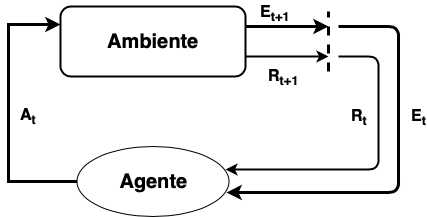
\includegraphics[width=.6 \textwidth]{conteudo/imgs/rl-diagram.png}
  \caption[Diagrama de aprendizagem por reforço]{Diagrama de aprendizagem por reforço. No \textit{loop} de \textit{feedback}, os subscritos indicam as etapas de tempo $t$ e $t + 1$, cada uma das quais se refere a estados diferentes: o estado no momento $t$ e o estado no momento $t + 1$. 
  A ação $A_t$ de um agente é determinada por sua \textbf{política}, que por sua vez é uma função que depende do estado atual do sistema $E_t$. A política de um agente tem como objetivo maximizar a \textbf{função de valor} que é calculada utilizando o \textbf{sinal de recompensa} $R_t$. O ambiente se comporta como um sistema caixa preta que transforma uma ação executada no estado atual $A_t$, no próximo estado $E_{t+1}$ e uma recompensa $R_{t+1}$
  }
  \label{rl-diagram-2}
 \end{figure}

 \subsection{Processos de Decisão de Markov e a Equação de Bellman} % (fold)
 \label{sub:processos_de_decisão_de_markov}
 % subsection processo_de_decisão_de_markov (end)


 \subsection{O Jogo} % (fold)
 \label{sub:o_jogo}

O jogo utilizado para teste do modelo foi o \textit{Frogger}. A escolha do mesmo foi feita tendo em vista sua simplicidade, tendo em vista as limitações de implementação (\textbf{Seção \ref{sub:limitacoes}}). A \textbf{Figura \ref{fig:frogg}} mostra o jogo utilizado. O objetivo do agente é partir do estado inicial mostrado na figura, e alcançar o topo da tela sem colidir com nenhum obstáculo.

\begin{figure}[h]
  \centering
  
\includegraphics[width=.6 \textwidth]{conteudo/imgs/frogg_ini_state.png}
  \caption[Jogo \textit{Frogger}]{Exemplo do jogo \textit{Frogger} utilizado. O jogador controla o quadrado verde no centro inferior da tela, enquanto os outros retângulos coloridos são os obstáculos}
  \label{fig:frogg}
 \end{figure}

 As recompensas para ações durante o jogo foram definidas inicialmente da seguinte forma:

 \begin{itemize}
 	\item $r=0$ caso o agente faça uma ação que o mantenha na mesma linha que se encontrava previamente;
 	\item $r=1$ caso o agente faça uma ação que o aproxime verticalmente de seu objetivo;
 	\item $r=-1$ caso o agente faça uma ação que o distancie verticalmente de seu objetivo;
 	\item $r=10$ caso o agente alcance seu objetivo.
 \end{itemize}

 % subsection o_jogo (end)
 

% section reinforcement_learning (end)

\section{Modelagem Matemática} % (fold)
\label{sec:modelagem_matematica}

Conforme descrito em \cite{play-atari-drl-deepmind}, são consideradas tarefas em que um agente interage com um ambiente $\varepsilon$, nesse caso o jogo em \textit{Allegro}, como uma sequência de ações, observações e recompensas. Em cada etapa de tempo, o agente seleciona uma ação em do conjunto de ações legais do jogo, $\mathcal{A} = \{1,\cdots ,K\}$. A ação é executada, modificando o estado e pontuação do jogo.
%Em geral, $\varepsilon$ pde ser estocástico.
O estado interno do jogo não é observado pelo agente, este observa apenas uma imagem $x_t \in \mathbb{R}^d$, que é um vetor de valores de pixel brutos que representam a tela do estado atual do jogo. Além disso, o agente recebe uma recompensa $r$ que representa a alteração na pontuação do jogo. 


É importante ressaltar que a pontuação do jogo pode depender de toda a sequência anterior de ações e observações. O feedback sobre uma ação só pode ser recebido depois de decorridos múltiplos de intervalos de tempo. Uma vez que o agente apenas observa as imagens da tela atual, a análise do atual estado do jogo pode ser mal-representada, ou seja, é difícil para o agente compreender totalmente a situação atual apenas da tela atual $x_t$. 
Para solucionar esse problema, considera-se como um estado $s_t$ do jogo, uma sequência de ações e observações $s_t = (x_{t-n},a_{t-n},\cdots,a_{t-1},x_t)$, as quais serão utilizadas para treinar o agente, fornecendo-o um melhor contexto do estado em que se encontra. Esse formalismo dá origem a um processo de decisão de Markov (MDP), no qual cada sequência é um estado distinto. Como resultado, podemos aplicar métodos de aprendizado por reforço padrão para MDPs, simplesmente usando a sequência completa $s_t$ como a representação do estado no tempo $t$.

O objetivo do agente é interagir com o jogo, selecionando ações de uma forma que maximize recompensas futuras. É feita a suposição padrão de que as recompensas futuras são descontadas por um fator de $\gamma$ por intervalo de tempo, e que o retorno descontado futuro é definido por: 
\begin{eqnarray}
	R_t=\sum_{t^{\prime}=t}^T \gamma^{t^{\prime}-t}\cdot r_{t^{\prime}}
\end{eqnarray}

onde T é o intervalo de tempo em que o jogo termina. 

A função de valor de ação ótima $Q^{*}(s, a)$ pode ser definida como o máximo retorno esperado alcançável de uma estratégia, depois de ver a sequência $s$ e se tomar alguma ação $a$:

\begin{eqnarray}
	Q^{*}(s, a)=max_\pi(\mathbb{E}[R_t | s_t=s,a_t=a,\pi])
\end{eqnarray}

onde $\pi$ é uma política que mapeia sequências para ações e $\mathbb{E}$ é a função de retorno esperado para um estado $s$ dado uma ação $a$.


A função de valor de ação ótima obedece a identidade da equação de Bellman. Essa se baseia na seguinte intuição: se o valor ótimo $Q^{*}(s_{t+1}, a_{t+1})$ da sequência $s_{t+1}$ na próxima etapa de tempo for conhecido para todas as ações possíveis ações $a_{t+1}$, então a estratégia ótima para o estado $s_t$ consiste em selecionar a ação $a_{t}$ que maximize o valor esperado futuro:

\begin{eqnarray}
	Q^{*}(s_t, a_t)= r + \gamma \cdot max(Q^{*}(s_{t+1},a_{t+1})|\forall a_{t+1})
\end{eqnarray}

A ideia básica por trás de muitos algoritmos de aprendizagem por reforço é estimar a função de valor de ação, usando a equação de Bellman como uma atualização iterativa. Assim, dado um fator de aprendizagem $\alpha$, o valor de $Q(s,a)$ é atualizado durante o treinamento da seguinte forma:

\begin{eqnarray}
	Q(s_t,a_t) = Q(s_t,a_t) + \alpha[r + \gamma\cdot max_{a_{t+1}}Q(s_{t+1},a_{t+1}) - Q(s_t,a_t)]
\end{eqnarray}

sendo que a subtração de $\gamma\cdot max_{a_{t+1}}Q(s_{t+1},a_{t+1})$ por $Q(s_t,a_t)$ é realizada para normalizar a atualização.

% section modelagem_matemática (end)

\section{Implementação} % (fold)
\label{sec:implementacao}

\subsection{Pré-processamento de Dados} % (fold)
\label{sub:preprocessamento}

% subsection préprocessamento (end)

\subsection{Limitações} % (fold)
\label{sub:limitacoes}

% subsection limitações (end)

% section implementação (end)
